\chapter{Implementation of the Graduated Cylindrical Shell model in Python}
\label{chp:GCS_Python}

The Graduated Cylindrical Shell model \citep[GCS,][]{Thernisien-2006-GCS,Thernisien-2011-GCS} is an empirical model that is commonly used to represent the three-dimensional structure of flux rope CMEs near the Sun. It defines a croissant-like 3D shape with conical legs whose ends are anchored to the center of the Sun, as shown in \autoref{fig:gcs_schematic}.

\begin{figure}
    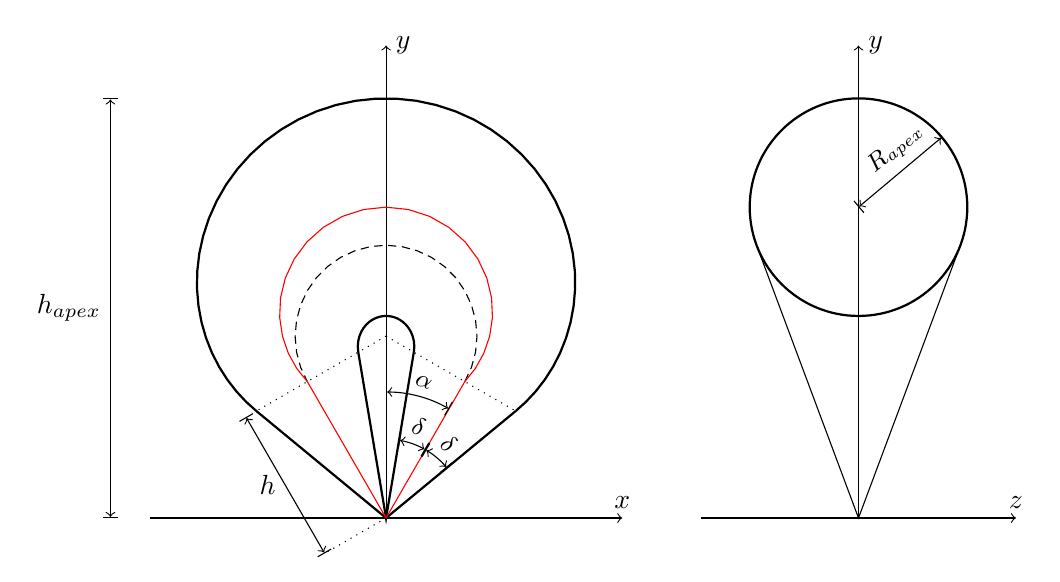
\begin{tikzpicture}
    \def\h{2}
    \def\palpha{30}
    \def\pkappa{0.35}
    
    \def\b{(\h / cos(\palpha))}
    \def\prho{(\h * tan(\palpha))}
    \def\pdelta{asin(\pkappa)}
    
    \def\Xnull{((\prho + \b * \pkappa^2 * sin(\x)) / (1 - \pkappa^2))}
    \def\Rc{sqrt(\Xnull^2 + (\b^2 * \pkappa^2 - \prho^2)/(1 - \pkappa^2))}
    
    \begin{scope}
        % xy view
        \draw[->] (0, 0) -- (0, 6) node[right] {$y$};
        \draw[->] (-3, 0) -- (3, 0) node[above] {$x$};
        
        \draw[densely dashed, domain=-\palpha:180+\palpha] plot ({\prho * cos(\x)}, {\prho * sin(\x) + \b});
        
        \draw[thick] ({90+\palpha+\pdelta}:{\h/cos(\pdelta)}) -- (0, 0) -- ({90-\palpha-\pdelta}:{\h/cos(\pdelta)});
        \draw[thick] ({90+\palpha-\pdelta}:{\h/cos(\pdelta)}) -- (0, 0) -- ({90-\palpha+\pdelta}:{\h/cos(\pdelta)});
        
        % central axis
        \draw[red] (90+\palpha:\h) -- (0, 0) -- (90-\palpha:\h);
        \draw[red, domain=-\palpha:180+\palpha] plot ({\Xnull * cos(\x)}, {\Xnull * sin(\x) + \b});
        
        \draw[thick,domain=-\palpha:180+\palpha,samples=50] plot ({(\Xnull + \Rc) * cos(\x)}, {(\Xnull + \Rc) * sin(\x) + \b});
        \draw[thick,domain=-\palpha:180+\palpha] plot ({(\Xnull - \Rc) * cos(\x)}, {(\Xnull - \Rc) * sin(\x) + \b});
        
        \draw[dotted] (0, {\b}) -- ({90+\palpha+\pdelta}:{\h/cos(\pdelta)});
        \draw[dotted] (0, {\b}) -- ({90-\palpha-\pdelta}:{\h/cos(\pdelta)});
        
        % definitions of delta, alpha, h and h_apex
        \draw[|<->|] ({90-\palpha-\pdelta}:{\h*0.5}) arc ({90-\palpha-\pdelta}:{90-\palpha}:{\h*0.5}) node[midway, above, rotate={-\palpha - \pdelta/2}] {\small$\delta$};
        \draw[|<->|] ({90-\palpha+\pdelta}:{\h*0.5}) arc ({90-\palpha+\pdelta}:{90-\palpha}:{\h*0.5}) node[midway, above, rotate={-\palpha + \pdelta/2}] {\small$\delta$};
        
        \draw[|<->|] ({90}:{\h*0.8}) arc ({90}:{90-\palpha}:{\h*0.8}) node[midway, above, rotate={-\palpha + \pdelta/2}] {\small$\alpha$};
        
        \def\x{90}
        \draw[|<->|] (0, 0) ++ ({\palpha}:-0.9) -- node[left] {$h$} ++({90+\palpha}:{\h});
        \draw[dotted] (0, 0) -- ++ ({\palpha}:-0.9);
        
        \draw[|<->|] (-3.5, 0) -- node[left] {$h_\text{apex}$} (-3.5, {\b + \Xnull + \Rc});
    \end{scope}
    
    \begin{scope}[xshift=6cm]
        % yz view
        \draw[->] (0, 0) -- (0, 6) node[right] {$y$};
        \draw[->] (-2, 0) -- (2, 0) node[above] {$z$};
        
        % front
        \def\Xnull{((\prho + \b * \pkappa^2 * sin(\x)) / (1 - \pkappa^2))}
        \def\Rc{sqrt(\Xnull^2 + (\b^2 * \pkappa^2 - \prho^2)/(1 - \pkappa^2))}
        \def\x{90}
        
        \draw[thick](0, {\b + \Xnull}) circle (\Rc);
        
        \draw ({90-\pdelta}:{(\b + \Xnull) * cos(\pdelta)}) -- (0, 0) -- ({90+\pdelta}:{(\b + \Xnull) * cos(\pdelta)});
        
        % definition of R_apex
        \draw[|<->|] (0, {\b + \Xnull}) -- node[above,rotate=40,xshift=1.5mm] {\small $R_\text{apex}$} ++ (40:{\Rc});
    \end{scope}
\end{tikzpicture}
    \caption[Illustration of the GCS model]{Illustration of the GCS model and definition of parameters $h_\text{apex}$, $\alpha$, $\delta$ and $R_\text{apex}$. Adapted from \citet{Thernisien-2011-GCS}. In this example, $\alpha = \SI{30}{\degree}$ and $\kappa = 0.35$.}
    \label{fig:gcs_schematic}
\end{figure}

The GCS geometry is constrained using 3 main parameters: The CME apex height $h_\text{apex}$ (or alternatively the leg height $h$), the angular half width $\alpha$, and the so-called aspect ratio $\kappa$, which corresponds to the half angle $\delta$ of the leg cones:
\begin{equation}
    \kappa = \sin \delta
\end{equation}
Three additional parameters describe the orientation of the flux rope relative to the Sun: The heliographic latitude $\theta$, longitude $\phi$ (typically in Stonyhurst or Carrington coordinates), and the tilt angle $\gamma$ (rotation around the $y$ axis in \autoref{fig:gcs_schematic}).

The GCS model is typically employed in a forward modelling approach, i.e. the model is visually compared to coronagraph observations of a CME and the input parameters iteratively adjusted by the scientist to achieve a good fit. This manual fitting process is ideally applied simultaneously to coronagraph images from multiple viewpoints, such as from the SOHO and STEREO spacecraft, to avoid ambiguity due to the line of sight effect. The resulting GCS parameters for the best fit can then be used for further evaluation, e.g. as input parameters for further models. Additional properties of the flux rope, such as the radius at the apex $R_\text{apex}$ (see \autoref{fig:gcs_schematic}) can also be calculated from these parameters, as derived by \citep{Thernisien-2011-GCS}. When applied to a sequence of consecutive images, the CME kinematics can also be reconstructed.

The original implementation of the GCS model in the Interactive Data Language (IDL) and a corresponding graphical user interface (GUI) was developed by \citet{Thernisien-2006-GCS} and is included in the under the name \texttt{scraytrace}\footnote{\url{https://hesperia.gsfc.nasa.gov/ssw/stereo/secchi/idl/scraytrace}} in the SolarSoft software package \citep{Freeland-1998-SolarSoft}. Using this implementation requires a local installation of SolarSoft and the corresponding database (SSWDB), which includes coronagraph images and calibration data. The setup process for these components for scientists that do not typically use IDL and SolarSoft is quite involved, and the GCS implementation is only partially documented and not very flexible, as it was initially hard-coded to work with STEREO-A and B data, with support for SOHO being manually added later.

The Python programming language is becoming increasingly popular in solar and heliospheric physics \citep[e.g.]{Burrell-2018}, and various open source software libraries to assist with the associated data analysis are available. Python is a modern general-purpose programming language that is easy to learn and emphasizes code readability. According to the TIOBE Programming Community Index\footnote{\url{https://www.tiobe.com/tiobe-index/}}, it has recently surpassed Java as the second most popular programming language, and in contrast to IDL, it is open source and available free of charge on all major operating systems.

The SunPy library \citep{sunpy_community2020}, which provides Python utilities to e.g. retrieve and plot solar images from various missions and to take care of the correct projection of plotted coordinates on top of these images, is one of the most widely-used Python toolkits for solar physics. However, it does not yet provide any models for CME reconstruction in coronagraph images.
Thus, I have developed an open source Python implementation of the GCS model and a simple GUI application. As it is easy to install and based on SunPy, it can not only be used as a standalone application, but also can also be integrated into existing Python-based plotting routines. The source code is available on GitHub at \url{https://github.com/johan12345/gcs_python}, and is also mirrored at Kiel University under \url{https://gitlab.physik.uni-kiel.de/ET/gcs_python}. It can be easily installed with the command
\begin{minted}{bash}
pip3 install git+https://github.com/johan12345/gcs_python.git
\end{minted}
(provided that Python 3.7 or above is already installed).

The following sections will describe the design and usage of this software package, and its validation against the original IDL version.

\section{GCS geometry}

The basic GCS geometry is implemented in the \texttt{gcs.geometry} package. This code is a close translation of the corresponding IDL routines from SolarSoft. Two basic functions are provided to calculate the geometry of the GCS structure based on the input parameters: The \texttt{skeleton} function (based on \texttt{shellskeleton.pro} in SolarSoft) calculates the shape of the central axis of the flux rope (thin solid line in \autoref{fig:gcs_schematic}), which consists of two straight segments in the legs and a curved segment in the front. The desired number of vertices along each part of the curve can be passed to the function.
In addition to the the points along the axis, the \texttt{skeleton} function also provides the radius of the circular shell at each point, and the orientation of these circles (i.e. the orientation of the tangent vector in the $xy$ plane).
The \verb|gcs_mesh| function (based on \texttt{cmecloud.pro} in SolarSoft) then uses the output of the \texttt{skeleton} function to construct a 3D mesh by generating circles around each point of the central axis with the appropriate radius and orientation. The parameters of the \verb|gcs_mesh| function are the half angle $\alpha$, the CME height $h_\text{apex}$, and the aspect ratio $\kappa$, as well as the desired numbers of vertices along the straight segments, along the front, and along each circle in the mesh.

% TODO: add plot here

In addition to these basic routines to construct the GCS mesh, there is also a function \verb|gcs_mesh_rotated|, which includes the 3 angles $\theta, \phi, \gamma$ to rotate the CME cloud in 3D space, and the function \verb|gcs_mesh_sunpy|, which converts the GCS mesh into a \texttt{SkyCoord} object, which contains the necessary metadata about the coordinate system so that the model can directly be integrated into a SunPy plot.

\section{Graphical user interface}

\section{Validation}
